\documentclass{article}

\usepackage{geometry}
\usepackage{makecell}
\usepackage{array}
\usepackage{multicol}
\usepackage{setspace}
\usepackage{changepage}
\usepackage{booktabs}
\usepackage{graphicx}
\usepackage{cprotect}
\usepackage{float}
\newcolumntype{?}{!{\vrule width 1pt}}
\newcommand{\paragraphlb}[1]{\paragraph{#1}\mbox{}\\}
\renewcommand\theadalign{tl}
\setstretch{1.10}
\setlength{\parindent}{0pt}

\geometry{top=12mm, left=1cm, right=2cm}
\title{\vspace{-1cm} WS24 Betriebssysteme Grundlagen Übung}
\author{Andreas Hofer}

\begin{document}
	\maketitle
	\section{Übung 3 - 07.11.2024}
	\subsection{Berechtigungen}
	Berechtigungen geben an, welche Nutzer welche Rechte für eine Datei besitzen. In Unix wird dabei zwischen dem Benutzer (u), der Gruppe (g) und Anderen (o) unterschieden.
	\begin{itemize}
		\item{Benutzer - u}
		\begin{itemize}
			\item{Der User, welche die Datei erstellt hat.}
		\end{itemize}
		\item{Gruppe - g}
		\begin{itemize}
			\item{Die Gruppe, zu welcher der User gehört.}
		\end{itemize}
		\item{Andere - o}
		\begin{itemize}
			\item{Others, also alle anderen.}
		\end{itemize}
	\end{itemize}
	Gleichzeitig gibt es die Berechtigungen read(r), write(w) und execute(x).
	\begin{itemize}
		\item{read (r)}
		\begin{itemize}
			\item{Die Berechtigung die Datei zu lesen und zu kopieren.}
		\end{itemize}
		\item{write (w)}
		\begin{itemize}
			\item{Die Berechtigung die Datei zu verändern, umzubenennen oder zu verschieben.}
		\end{itemize}
		\item{execute (x)}
		\begin{itemize}
			\item{Die Berechtigung die Datei auszuführen, was nur bei .exe oder Skriptdateien relevant ist. Zum Ausführen von Skriptdateien wird zusätzlich eine Leseberechtigung benötigt, da der Interpreter die Datei lesen muss um sie ausführen zu können.}
		\end{itemize}
	\end{itemize}
	Zusätzlich gibt es in Linux die Angabe des Filetyps.
	\begin{itemize}
		\item{-}
		\begin{itemize}
			\item{Eine reguläre Datei}
		\end{itemize}
		\item{d}
		\begin{itemize}
			\item{Ein Ordner (directory)}
		\end{itemize}
		\item{l}
		\begin{itemize}
			\item{Eine Verknüpfung (Symbolic Link)}
		\end{itemize}
		\item{p}
		\begin{itemize}
			\item{Eine named pipe. Kann bei bash scripts verwendet werden.}
		\end{itemize}
	\end{itemize}
	Die Berechtigungen in Linux werden stets als eine Folge an Zeichen für jede Datei angegeben, wobei die Folge die Berechtigungen angibt. \\
	\begin{figure}[H]
	\centering
	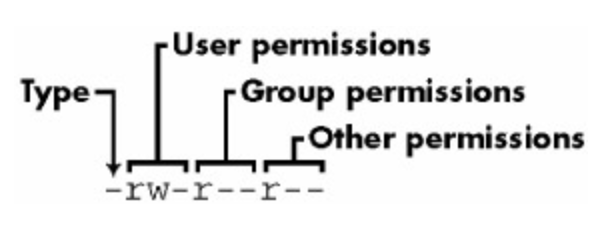
\includegraphics[scale=0.5]{Bilder/permissions.png}
	\caption{Illustration der UNIX Berechtigungen}
	\end{figure}
	Dabei gibt das erste Zeichen die Art der Datei an. Dabei muss beachtet werden, dass obwohl der Bindestrich - hier als Datei gilt, hat er in weiterer Folge eine andere Bedeutung. Als nächstes werden jeweils die Berechtigungen des Benutzers, welchem die Datei gehört, der Gruppe, zu welcher der User gehört, und allen anderen in einer Gruppe aus drei Zeichen angegeben, welche jeweils die Lese-, Schreib- und Ausführberechtigungen angeben. Wenn, eine Berechtigungsangabe zum Beispiel so aussieht: \verb|-rw-r-----|, dann bedeutet das, dass es eine Datei ist \verb|-|, der Benutzer Lese- und Schreibe- aber keine Ausführungsberechtigungen hat \verb|rw-|, die Gruppe nur Leseberechtigungen hat \verb|r--| und alle anderen keine Rechte besitzen \verb|---|. 
	\subsection{chmod}
	Mit dem Befehl \verb|chmod| kann man Rechte von Dateien anpassen. Dabei gibt es einen numerischen und einen symbolischen Weg um diesen anzugeben.
	\subsubsection{Numerisch}
	Bei der numerischen Variante wird jedem der drei Berechtigungen eine Zahl zugeordnet: \\ \\
	\begin{tabular}{| c | c | c |}
	 	\toprule
	 	execute & write & read \\ \midrule
	 	1 & 2 & 4 \\
	 	\bottomrule
	 \end{tabular} \\
	 Dabei werden die Berechtigungen kombiniert, indem man die Zahlen der Berechtigungen addiert, was erklärt, wieso read den Wert 4 hat. So ergibt sich, dass man bei der Angabe der Zahl 7, alle Berechtigungen vergibt und bei 0 keine: \\
	 \begin{tabular}{| c | c |}
	 	\toprule
	 	Nummer & Äquivalent\\ \midrule
	 	0 & --- \\
	 	1 & --x \\
	 	2 & -w- \\
	 	3 & -wx \\
	 	4 & r-- \\
	 	5 & r-x \\
	 	6 & rw- \\
	 	7 & rwx \\ \hline
	 \end{tabular}
	\section{Übung 5 - 20.11.2024}
	\subsection{Dateien einlesen}
	Zusätzlich zu dem Umleiten des outputs eines Programms in ein File, kann man auch stattdessen ein File als input für einen Befehl angeben. Dazu muss man das kleiner Zeichen (<) verwenden. \verb|wc -l < f1.txt| -> f1.txt enthält 5 Zeilen, welche sofort eingelesen wird und deshalb 5 ausgibt. 
	\subsection{Standard In-/Output/Error}
	Der PC hat immer einen Standard Input, einen Standard Output und einen Standard Error definiert. Der Standard Input ist normalerweise die Tastatur und sowohl der Standard Output als auch der Standard Error die Konsole. Diese Einstellungen sind als Dateideskriptoren reserviert und können mit den Zeichen 0, 1 und 2 verändert werden. Wenn man also zum Beispiel \verb|ls 2> f1.txt| eingibt, würde ls, im Falle eines Fehlers seinen Output nicht an die Konsole ausgeben sondern in das file f1.txt schreiben. 
	\cprotect\subsection{\verb|exec|}
	Die Dateideskriptoren muss man normalerweise bei jeder Operation explizit angeben und sie halten sich nicht. Falls man das will, kann man den Befehl \verb|exec| vor dem Befehl angeben, um so den Deskriptor für die Dauer des Skripts abzuändern. 
	\subsection{Vergleiche}
	Um in Bash zwei Werte miteinander zu vergleichen benötigt man die eckige Klammer \verb|[]|. Die Operatoren innerhalb dieser Klammer werden dann zu einem Wahrheitswert reduziert. Dabei muss man sicherstellen, dass stets nach der Ersten und vor der zweiten Klammer ein Leerzeichen steht, da der Interpreter sonst eine Fehlermeldung ausgibt: \verb|[ a1 -ne b1 ]|  
	\subsubsection{Arithemtische Vergleiche}
	Anders als in Java kann man in Bash für integer keine Vergleiche mit \textit{<} oder \textit{>} oder \textit{==} durchführen (Ohne doppelte eckige Klammern zu verwenden \verb|[[]]|. Dabei sollte man stets im Kopf behalten, dass in bash 0 \verb|true| und alles andere als \verb|false| interpretiert wird. Stattdessen gibt es Befehle, welche die gleiche Aufgabe haben:
	\begin{itemize}
		\item{\verb|-eq| (\textbf{eq}ual)}
		\begin{itemize}
			\item{Wahr wenn die beiden Terme gleich sind}
		\end{itemize}
		\item{\verb|-ne| (\textbf{n}ot \textbf{eq}ual)}
		\begin{itemize}
			\item{Wahr, wenn die beiden Terme nicht gleich sind.}
		\end{itemize}
		\item{\verb|-gt| (\textbf{g}reater \textbf{t}han)}
		\begin{itemize}
			\item{Wahr, wenn der rechte Term \textbf{größer} als der linke ist.}
		\end{itemize}
		\item{\verb|-ge| (\textbf{g}reater \textbf{e}qual)}
		\begin{itemize}
			\item{Wahr, wenn der rechte Term \textbf{größer oder gleich} groß ist.}
		\end{itemize}
		\item{\verb|-lt| (\textbf{l}ss \textbf{t}han)}
		\begin{itemize}
			\item{Wahr, wenn der rechte Term \textbf{kleiner} ist.}
		\end{itemize}
		\item{\verb|-le| (\textbf{l}ess \textbf{e}qual)}
		\begin{itemize}
			\item{Wahr, wenn der rechte Term \textbf{kleiner oder gleich} groß ist.}
		\end{itemize}
	\end{itemize}
	\subsubsection{Vergleiche von Zeichenketten}
	Man kann auch Zeichenketten wie Strings miteinander vergleichen
	\subsection{If/Then}
	If Konstruke Funktionieren größenteils gleich als in Java, haben jedoch ein paar syntaktische Unterschiede. \\
	Gleich wie in den Vergleichen, muss auch für den Vergleich in ifs ein Paar eckige Klammern verwendet werden. Zusätzlich braucht man danach ein \verb|then| und zum Abschluss des Konstrukts ein \verb|fi|:
	\begin{verbatim}
	  if [ condition ]
	  then
	  	command1
	  else
	  	command2
	  fi
	\end{verbatim} 
	Falls man ein else und ein if kombinieren möchte, kann man ein \verb|elif| verwenden, was die beiden Wörter verbindet.
	\section{Übung 6 - 21.11.2024}
	\cprotect\subsection{\verb|for|}
	Eine \verb|for| Schleife funktioniert in bash praktisch gleich wie in anderen Programmiersprachen. Dabei gibt es gleich wie in Java entweder über eine Liste oder ein Array iterieren (Sequenziell durchlaufen) oder mit einer Laufvariable eine bestimmte Menge an Durchläufen zu vollführen. Wenn es sich um eine Liste oder ein Array handelt, kann die for Schleife wie folgt aussehen, wobei args jedes Element der Liste in Folge durchlaufen wird und list die relevante Liste darstellt.
	\begin{verbatim}
	 for <args> in <list>
	 do
	   <command>
	 done
	 \end{verbatim} 
	 Wenn man eine Zählvariable definieren will, kann man diese stattdessen im Stil einer C-Schleife schreiben. Dabei muss man die Argumente jedoch in zwei Klammern \verb|(())| setzen. 
	 \begin{verbatim}
	 for (( i=0; i<4;i++)); do
	   <command>
	 done
	 \end{verbatim} 
	 \subsubsection{Wildcards}
	 Man kann Wildcards wie \verb|*| auch innerhalb von Schleifen wie for verwenden. Zum Beispiel wählt eine for Schleife, welche die Wildcard \verb|*.txt| löscht, bei jeder Iteration eine Datei mit der Endung .txt in dem Ordner. Dateien werden dabei in alphabetischer Folge ausgewählt:
	 \begin{verbatim}
	 let file = ../B2/*.txt
	 for i in $file
	 do
	 	rm $i
	 done
	 \end{verbatim}
	 \cprotect\subsection{\verb|while|}
	 Gleich wie for Schleifen, existieren auch \verb|while| Schleifen, mit sehr ähnlicher funktionsweise als in anderen Programmiersprachen. Dabei muss jedoch, anders als bei der for Schleife, der abgefragte Wert in eckigen Klammern [] sein:
	 \begin{verbatim}
	 input="hello"
	 while [ $input != "bye" ]
	 do 
       <commands>
	 done
	 \end{verbatim}
	 Eine Sache, welche man bei while Schleifen im Auge behalten sollte ist, dass bash nur Strings mit Strings vergleichen kann, was durch den Umstand, dass es weakly-typed (Der Compiler entscheidet welchen Variablentypen es verwendet) ist, erschwert wird. So muss man explizit eine String Variable mit zwei Anführungszeichen generieren um diese innerhalb der while Schleife vergleichen zu können.
	\cprotect\subsection{\verb|break| und \verb|continue|}
	\verb|break| und \verb|continue| können verwendet werden um den Ablauf der for und while Schleife zu manipulieren. Da beide Schleifen erst am Ende ihres Blocks erneut überprüfen ob die Bedingung noch gegeben ist, ist es manchmal eine gute Idee schon davor die Schleife abzubrechen oder direkt zur nächsten Iteration zu springen. Dabei kann \verb|break| verwendet werden um sofort die momentane Schleife zu beenden und mit dem Code danach weiterzumachen. \verb|continue| hingegen bricht die Ausführung der momentane Iteration ab und beginnt sofort mit der nächsten, bleibt jedoch innerhalb der Schleife (Außer die Iteration war bereits die letzte.)
	\section{Übung 6 - 27.11.2024}
	\subsection{Funktionen}
	Funktionen können verwendet werden um gewissen Code auszulagern um diesen später (eventuell häufiger) wiederzuverwenden. In bash kann eine Funktion zwar einen Rückgabewert haben, dieser muss jedoch numerisch sein, weshalb man keine Strings zurückgeben kann. \\
	Da Bash interpretiert wird müssen Funktionen jedoch vor dem ausgeführten Code angegeben werden da Bash nur einen passthrough hat. \\
	\subsubsection{Syntax}
	Bash Funktionen können in drei verschiedenen Wegen angegeben werden. \\
	Entweder mit dem keyword \textbf{function} gefolgt von eckigen Klammern:
	\begin{verbatim}
	function <function_name> {
		<code>
	}
	\end{verbatim}
	Alternativ kann man statt function auch runde Klammern verwenden.Diese dienen jedoch \textbf{nicht} um Parameter zu übergeben sondern existieren um dem Interpreter mitzuteilen, dass es sich um eine Funktion handelt:
	\begin{verbatim}
	<function_name> () {
		<code>
	}
	\end{verbatim}
	Man kann diese beiden Arten auch kombinieren, und sowohl function als auch die Klammern schreiben:
	\begin{verbatim}
	function <function_name> () {
		<code>
	}
	\end{verbatim}
	
\end{document}